\documentclass{MO824}
\usepackage[utf8]{inputenc}
\usepackage[brazil]{babel}      % para texto em Português
\usepackage{amsfonts}
\usepackage{amsmath,amssymb}
\usepackage{graphicx}
\usepackage{xcolor}
\usepackage{hyperref}
\usepackage{multirow}
\usepackage{algorithmic}
\usepackage{subfig}
\usepackage[ruled, vlined, portuguese]{algorithm2e}
\usepackage[]{lpform}

% Commands
\newcommand{\Z}{\mathbb{Z}}
\newcommand{\B}{\mathbb{B}}
\newcommand{\N}{\mathbb{N}}
\newcommand{\R}{\mathbb{R}}
\renewcommand{\lpsubjectto}{s.a.}

\title{Atividade 9 - Grupo 3 - MO824}

\author{
    Ana Clara Zoppi Serpa   - RA 165880\\
    Victor Ferreira Ferrari - RA 187890
}

\begin{document}    

    



\criartitulo

\runningheads{A.C.Z. Serpa e V.F. Ferrari}%
{Atividade 9}

\begin{abstract}
{\bf Resumo}. Este trabalho consiste de um estudo de caso para o problema de alocação de professores (PAP). É apresentado um modelo matemático para o problema, e é implementada uma solução heurística baseada no GRASP. A solução direta do modelo com o resolvedor Gurobi foi comparada à metaheurística por meio de perfis de desempenho e tabelas, e os resultados mostram que o Gurobi teve melhor desempenho para este problema, tanto quanto à otimalidade das soluções como ao tempo necessário para encontrá-las. A metaheurística implementada obteve resultados que em geral se aproximam pouco do ótimo. Das configurações testadas, o GRASP com viés linear e $\alpha=0.1$ foi a melhor.

{\bf Palavras-chave}. Otimização, alocação, PAP, metaheurística, GRASP, PLI

\end{abstract}

\section{Introdução}
    \paragraph*{}
    Este trabalho consiste de um estudo do problema de alocação de professores (PAP), proposto na Atividade 9 de MO824 2S-2020. Um modelo matemático é apresentado, além da implementação de uma metaheurística. Os métodos são comparados por meio de perfis de desempenho e tabelas.
    
    \subsection{Problema} \label{problem}
    O Problema de Alocação de Professores (PAP) consiste em encontrar uma alocação de $P$ docentes em $D$ disciplinas, que devem ser distribuídas em períodos da semana, tal que certas restrições sejam satisfeitas. Dada a avaliação $a_{pd} \in [0,100]$ do professor $p$ referente a uma disciplina $d$, o objetivo é maximizar as avaliações correspondentes aos pares $(professor,disciplina)$ alocados. 
    
    Cada disciplina exige $h_d \in [1,3]$ períodos em uma semana. Cada semana é dividida em cinco dias, e cada dia é separado em quatro períodos. Ou seja, cada semana contém $T=20$ períodos, que são numerados em ordem cronológica. Não mais que $S$ disciplinas podem ser ministradas no mesmo período, sendo $S$ o número de salas do instituto.
    
    Cada professor possui restrições sobre os períodos, ou seja, se $r_{pt}=1$, o professor $p$ pode lecionar no período $t$, e vice-versa. Um professor pode somar até $H=3$ períodos na semana, e não pode lecionar mais de uma disciplina no mesmo período. Caso uma disciplina não possa ser alocada, uma penalidade de $-100$ é aplicada na função objetivo.
    
\section{Modelo Matemático}
    As seguintes variáveis foram usadas no modelo:
    
    $x_{pd}$: Variável de decisão binária associada à alocação ($x_{pd}=1$) ou não ($x_{pd}=0$) do professor $p$ na disciplina $d$.\\
    
    $y_d$: Variável binária associada à alocação ($y_d = 1$) ou não ($y_d = 0$) de uma disciplina (em qualquer período).\\
    
    $z_{pt}$: Variável binária associada à alocação ($z_{pt}=1$) ou não ($z_{pt}=0$) do professor $p$ no período $t$.
    
    \begin{lpformulation}[(PAP)]
        \lplabel{lp:PAP}
        \lpobj[FO]{max}{\sum_{d=1}^D \sum_{p=1}^P a_{pd}x_{pd} - \sum_{d=1}^D 100(1-y_d)}
        \lpeq[1]{\sum_{p=1}^P x_{pd} = y_d}{d \in \{1\dots D\}}
        \lpeq[4]{\sum_{p=1}^P z_{pt} \leq S}{t \in \{1\dots T\}}
        \lpeq[5]{z_{pt} \leq r_{pt}}{p \in \{1\dots P\}, t \in \{1\dots T\}}
        \lpeq[6]{\sum_{t=1}^T z_{pt} \leq H}{p \in \{1\dots P\}}
        \lpeq[3/7]{\sum_{t=1}^T z_{pt} = \sum_{d=1}^D h_dx_{pd}}{p \in \{1\dots P\}}
        \lpeq[dom]{x_{pd}, y_{d}, z_{pt} \in \B}{p \in \{1\dots P\}, d \in \{1\dots D\}, t \in \{1\dots T\}}
    \end{lpformulation}
    
    onde, como descrito na Seção \ref{problem}, $D$ é a quantidade de disciplinas que necessitam de alocação, $P$ é a quantidade de professores disponíveis, $S$ é a quantidade de salas disponíveis por período, e há $T=20$ períodos disponíveis por semana. $a_{pd}$ é a avaliação do professor $p$ na disciplina $d$, $h_d$ é a carga horária semanal (em períodos) exigida pela disciplina $d$, e $r_{pt}$ é a disponibilidade do professor $p$ no período $t$. A carga horária máxima $H$ de um professor é de 3 períodos.
    
    A função objetivo \eqref{FO} procura maximizar a soma das avaliações dos professores nas disciplinas em que são alocados, com uma penalização se a disciplina não foi alocada.
    
    A restrição \eqref{1} indica que, se uma disciplina for alocada, há exatamente um professor ligado a ela (já que $y_d$ também é binária). A restrição \eqref{4} limita o número de disciplinas em um período pelo número de salas.
    
    A restrição \eqref{5} indica que um professor só é alocado em um período se estiver disponível nele. A carga horária de um professor é limitada em $H=3$ períodos na restrição \eqref{6}. Finalmente, a restrição \eqref{3/7} certifica que um professor leciona no máximo 1 disciplina por período, ou seja, o número de períodos em que um professor está alocado é a soma da carga horária das disciplinas ministradas por ele, e a restrição \eqref{dom} restringe o domínio das variáveis.
    
    A função objetivo pode ser simplificada para:
    \begin{equation}
        \max~\sum_{d=1}^D (100y_d + \sum_{p=1}^P a_{pd}x_{pd}) - 100D
    \end{equation}
    
    A variável $y$ também é desnecessária, e pode ser removida do modelo, se a substituirmos pelo somatório da restrição \eqref{1}. Ao substituir e simplificar, a nova função objetivo e restrições alteradas (equivalentes às restrições \eqref{1} e \eqref{dom}) são:
    
    \begin{lpformulation}[(PAP\_ALT)]
        \lplabel{lp:PAPALT}
        \lpobj[FO_ALT]{max}{\sum_{d=1}^D (\sum_{p=1}^P (a_{pd}+100)x_{pd}) - 100D}
        \lpeq[1_ALT]{\sum_{p=1}^P x_{pd} \leq 1}{d \in \{1\dots D\}}
        \lpeq[dom_ALT]{x_{pd}, z_{pt} \in \B}{p \in \{1\dots P\}, d \in \{1\dots D\}, t \in \{1\dots T\}}
    \end{lpformulation}
    
    O modelo ainda contém as restrições \eqref{4}, \eqref{5}, \eqref{6} e \eqref{3/7}.
    
\section{Metaheurística} \label{method}

Neste trabalho foi implementado o GRASP (\emph{greedy randomized adaptive search procedure}) \cite{grasp} para solucionar o problema, que consiste de uma metaheurística iterativa na qual cada iteração possui uma fase construtiva seguida de uma busca local. Em linhas gerais, uma solução é construída na primeira etapa e sua vizinhança é investigada na segunda, visando encontrar uma solução de melhor custo.

    \subsection{Heurística Construtiva}

    Na heurística construtiva, os elementos candidatos a entrarem na solução são avaliados de forma gulosa no que diz respeito aos seus custos de inserção: quanto maior esse custo, mais próximo do máximo a solução se encontra. A cada iteração, um dos elementos (factíveis) é escolhido para a solução.
    
    No entanto, para ampliar a variância entre iterações, ao invés de selecionarmos o elemento cujo custo $c$ melhor afeta a solução, concebemos uma lista de candidatos restrita (RCL, do inglês Restricted Candidate List), que engloba todos elementos com custo no intervalo $[c^{\text{min}}, c^{\text{min}} + \alpha \cdot (c^{\text{max}} - c^{\text{min}})]$. Um membro da RCL é, então, selecionado aleatoriamente (como detalhado na Seção \ref{random}) para ingressar na solução, e o processo se repete enquanto a inserção de um candidato melhorar a solução ou a lista de candidatos esvaziar. Note que o parâmetro $\alpha$ controla o quão guloso ou aleatório é o algoritmo.

    \subsubsection{Função de Viés (\textit{Bias})} \label{random}

    Nessa abordagem, a escolha aleatória de um candidato da RCL a ser inserido na solução em construção é feita a partir de uma \textbf{função de viés}. Nela, são atribuídas probabilidades para cada elemento com base em uma função $\texttt{bias}(r)$ e no valor de inserção do elemento na solução. 
    
    Dado um candidato $\sigma$, podemos definir um \textit{rank} $r(\sigma)$ para o elemento dentro do conjunto $C$. Assim, a probabilidade de $\sigma$ é dada pela Equação \eqref{bias}.
    
    \begin{equation} \label{bias}
        \pi(\sigma) = \frac{\texttt{bias}(r(\sigma))}{\sum_{\sigma' \in C} \texttt{bias}(r(\sigma'))}
    \end{equation}
    
    Esse método não elimina diversidade, pois a escolha ainda é feita aleatoriamente, mas fornece um viés para essa escolha, tentando aumentar a qualidade média das soluções.
    
    A escolha padrão do GRASP ainda pode ser feita, definindo a função \texttt{bias} constante igual a 1, independente do \textit{rank}, e assim as probabilidades são iguais para todos os elementos da RCL. Porém, outras combinações podem ser testadas, como funções lineares, logarítmicas, exponenciais e polinomiais \cite{grasp}. Após diversos testes com todas as funções citadas, escolhemos focar em uma função de viés \textbf{linear} (além da padrão).

    \subsection{Busca Local}
    A etapa de busca local consiste na exploração da vizinhança da solução $S$ construída anteriormente. Uma vizinhança imediata consiste nas soluções obtidas ao \textbf{inserir} ou \textbf{remover} um elemento em $S$, ou \textbf{trocar} um elemento de $S$ por outro. Essas operações são chamadas de \textit{movimentos de vizinhança}. A lista de candidatos é atualizada a cada iteração, para conter apenas elementos factíveis. O processo de atualização da CL e os movimentos de vizinhança podem ser vistos na Seção \ref{model}.
    
    Dados os movimentos, a vizinhança é explorada até que um ótimo local seja encontrado, sendo este retornado para atualização da solução titular. Essa busca segue a estratégia \textit{best-improving}, que trata de avaliar todos os movimentos possíveis a partir da solução atual, e escolher aquele que fornecer o melhor custo. Em outras palavras, todas as inserções, remoções e trocas são avaliadas, e o melhor movimento é escolhido. 
    
    \subsection{Modelagem do Problema} \label{model}
    
    Cada elemento da solução é um par $(p,d)$, o que equivale à decisão de que um professor $p$ lecionará a disciplina $d$. Além disso, outras estruturas auxiliares são usadas para armazenar as combinações $(d,t)$, ou seja, a alocação das disciplinas $d$ nos períodos $t$ disponíveis, para verificação de viabilidade das soluções.
    
    O operador de inserção consiste em alocar um professor $p$ a uma disciplina $d$, e alocar os períodos necessários por \emph{first-fit} --- ou seja, no primeiro período disponível. O operador de remoção envolve remover um professor de disciplina, e seus períodos. O operador de troca consiste em uma remoção seguida de uma inserção.
    
    A cada iteração da heurística construtiva e da busca local, um processo de viabilização da lista de candidatos é feito. A CL é reiniciada, e para cada disciplina que ainda não foi alocada, todos os pares $(p,d)$ possíveis são avaliados quanto à viabilidade, seguindo as restrições do modelo (PAP\_ALT). Assim, um elemento só está na lista de candidatos se sua inserção é segura.
    
    A presença das estruturas auxiliares permite a expansão da solução final, para incluir todas as triplas $(p,d,t)$.

\section{Implementação e Avaliação}
    A implementação da solução heurística foi feita em \emph{Java}, com base nos \textit{frameworks} fornecidos, com as modificações citadas na Seção \ref{method} e outras necessárias para obtenção dos dados e realização dos experimentos. Foi utilizado como \textit{software} de resolução dos modelos matemáticos o \textit{solver} Gurobi Optimizer V9.0.3, com a API para \emph{Java}.
    
    Dois modelos para o problema foram implementados: ``GUROBI'' se refere ao uso do modelo com as variáveis $y_d$ para o PAP (modelo PAP), e ``GUROBI ALT'' se refere ao uso do modelo no qual as variáveis $y_d$ são substituídas pelo somatório (modelo PAP\_ALT). Quatro configurações do GRASP foram testadas:
    
    \begin{enumerate}
        \item PADRÃO: $\alpha_1=0.25$, e \textit{bias} aleatório.
        \item PADRÃO+LINEAR: $\alpha_1=0.25$, e \textit{bias} linear.
        \item PADRÃO+LINEAR+ALPHA2: $\alpha_2=0.1$, e \textit{bias} linear.
        \item PADRÃO+LINEAR+ALPHA3: $\alpha_3=0.4$, e \textit{bias} linear.
    \end{enumerate}

    Todos os métodos foram executados com limite de 1800 segundos (30 minutos) e sem limite de memória. Para o GRASP, o máximo de iterações em todos os experimentos foi 1000. As instâncias utilizadas em nossos experimentos foram fornecidas previamente no pacote da atividade. 
    
    As especificações de hardware do computador no qual foram feitas as execuções estão na \tablename~\ref{table:conditions}. O sistema operacional utilizado foi o Windows 10 (64 bits).
    
        \begin{table}[ht]
            \centering
            \caption{Condições de Execução}
            \label{table:conditions}
            \vspace{0.3cm}
            \resizebox{70ex}{!}{
            \begin{tabular}{|c|c|}
            \hline
                Modelo da CPU & Intel(R) Core(TM) i7-7500 CPU\\ \hline
                Frequência do Clock da CPU & 2.70 GHz - 2.90 GHz \\ \hline
                RAM & 8,00 GB/2133 MHz \\
            \hline
            \end{tabular}
            }
        \end{table}

\section{Resultados e Análise}

A tabela \ref{tab-gurobi} mostra os resultados obtidos com o resolvedor Gurobi para cada instância, sendo as colunas LB e UB referentes aos limitantes inferior e superior indicados pelo resolvedor para o custo (valor da função objetivo) da solução, respectivamente. O tempo de execução foi medido em segundos. Os casos em que a solução encontrada é ótima estão destacados em negrito na tabela \ref{tab-gurobi}. 

Os resultados para a resolução direta dos modelos foram muito bons. Foram encontradas soluções ótimas para todas as instâncias com o modelo GUROBI. Já com GUROBI\_ALT, não foi possível confirmar a otimalidade das soluções para as instâncias P50D50S3 e P100D150S10, no tempo alocado. Ainda assim, as soluções adquiridas são ótimas. Quanto ao tempo de execução, o modelo GUROBI foi mais lento que o modelo GUROBI\_ALT somente para a instância P100D150S20. Esses resultados sugerem que o modelo com as variáveis $y_d$ é melhor tanto em termos de tempo de execução quanto na capacidade de encontrar soluções garantidamente ótimas para o problema PAP.

As Tabelas \ref{tab-grasp-1} e \ref{tab-grasp-2} mostram os resultados obtidos com a metauheurística GRASP para os diferentes valores de $\alpha$ (0.1, 0.25, 0.4) e as funções de viés (linear e aleatória) exploradas. As configurações, salvo dois casos, ultrapassaram o limite de 30 minutos estipulado para a execução. 

Em geral, os resultados do GRASP não alcançaram os modelos em termos de qualidade. Nenhuma solução ótima foi encontrada, embora nas configurações com viés linear soluções próximas das ótimas tenham sido encontradas para algumas instâncias. O valor $\alpha = 0.1$ com bias linear parece ter sido a melhor abordagem, obtendo soluções mais próximas das ótimas pontadas pelo resolvedor Gurobi em mais instâncias do que as demais configurações.

\begin{figure}[ht]
    \centering
    \subfloat[Escala Linear]{
    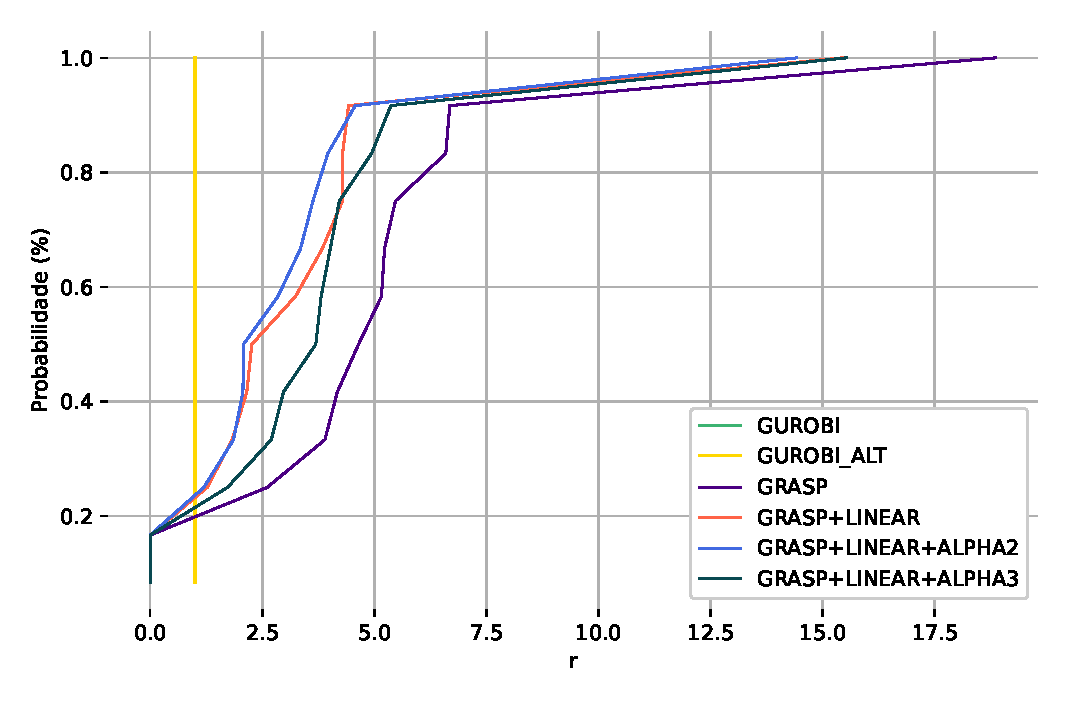
\includegraphics[width=0.5\textwidth, angle=0]{PP/objectiveFunction.eps}
    }
    \subfloat[Escala Log]{
    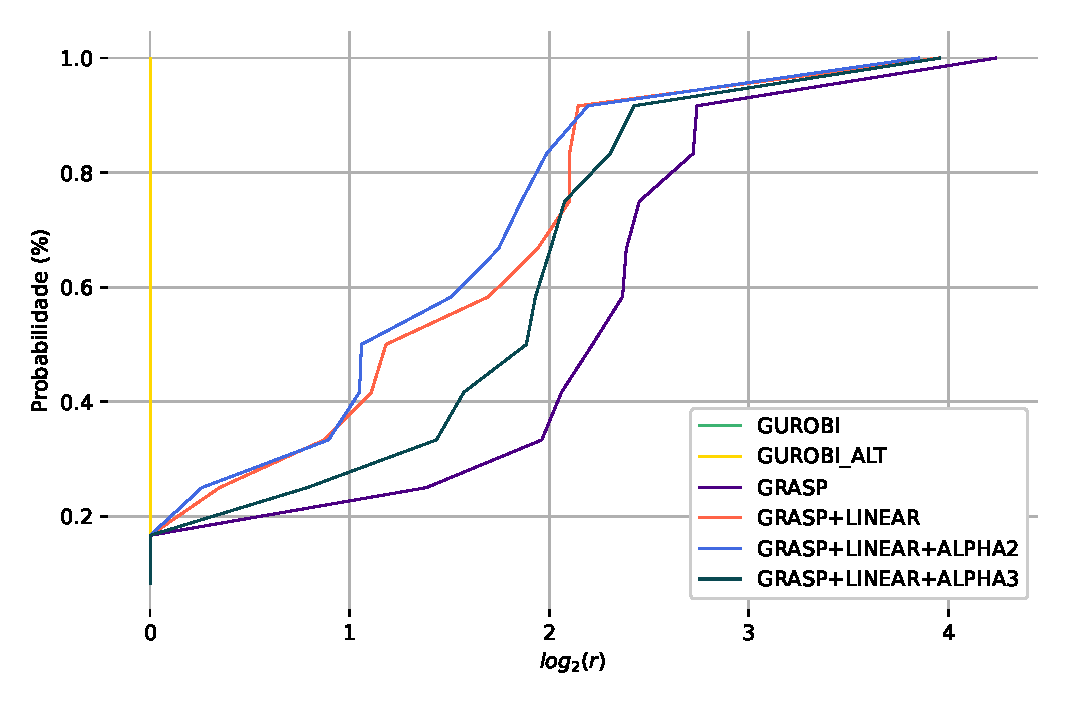
\includegraphics[width=0.5\textwidth, angle=0]{PP/objectiveFunctionLog.eps}
    }
    \caption{Perfis de Desempenho (Função Objetivo)}
    \label{fig:pp_obj}
\end{figure}

A Figura \ref{fig:pp_obj} contém a análise de perfis de desempenho para todos os métodos testados. Pode-se ver que as curvas dos modelos (sobrepostas) claramente dominam as outras, atingindo as melhores soluções em todas as instâncias. Entre os métodos heurísticos, se confirma a conclusão anterior: a configuração com viés linear e $\alpha=0.1$ tem a curva dominante. Por outro lado, a configuração com viés aleatório retornou a pior curva, ou seja, a mudança no viés melhorou consideravelmente a qualidade das soluções encontradas.

Isso sugere que o método implementado pode ser melhorado, seja com outros métodos alternativos de construção (já que as funções de viés foram bem-sucedidas) ou com mudanças na modelagem do problema. Seria interessante explorar outras formas de lidar com a alocação dos períodos nos operadores de busca local, em vez de utilizar \emph{first-fit}, seja com aleatoriedade ou uma heurística mais sofisticada.

Em conclusão, comparando os dois métodos estudados (GRASP e Gurobi), o resolvedor Gurobi teve um desempenho claramente melhor, tanto em termos de qualidade das soluções encontradas como de tempo de execução.


\begin{table}[ht]
\centering
\caption{Resultados obtidos com o resolvedor Gurobi}
\label{tab-gurobi}
\begin{tabular}{|l|c|c|c|c|c|c|}
\hline
            & \multicolumn{3}{c|}{GUROBI}                 & \multicolumn{3}{c|}{GUROBI\_ALT}                \\ \hline
Instância   & LB             & UB             & Tempo (s) & LB               & UB               & Tempo (s) \\ \hline
P50D50S1    & \textbf{-1292} & \textbf{-1292} & 0.062     & \textbf{-1292} & \textbf{-1292} & 0.062     \\ \hline
P50D50S3    & \textbf{2271}  & \textbf{2271}  & 3.452     & 2271           & 2371           & 1800.079  \\ \hline
P50D50S5    & \textbf{4770}  & \textbf{4770}  & 0.141     & \textbf{4770}  & \textbf{4770}  & 1.875     \\ \hline
P70D70S1    & \textbf{-3058} & \textbf{-3058} & 0.062     & \textbf{-3058} & \textbf{-3058} & 0.421     \\ \hline
P70D70S3    & \textbf{924}   & \textbf{924}   & 1.109     & \textbf{924}   & \textbf{924}   & 10.123    \\ \hline
P70D70S5    & \textbf{4265}  & \textbf{4265}  & 0.219     & \textbf{4265}  & \textbf{4266}  & 2.609     \\ \hline
P70D100S6   & \textbf{4610}  & \textbf{4610}  & 0.437     & \textbf{4610}  & \textbf{4610}  & 2.890     \\ \hline
P70D100S8   & \textbf{7177}  & \textbf{7177}  & 1.719     & \textbf{7177}  & \textbf{7177}  & 49.316    \\ \hline
P70D100S10  & \textbf{9616}  & \textbf{9617}  & 4.671     & \textbf{9616}  & \textbf{9617}  & 23.245    \\ \hline
P100D150S10 & \textbf{7626}  & \textbf{7626}  & 315.613   & 7626           & 7743           & 1800.248  \\ \hline
P100D150S15 & \textbf{13259} & \textbf{13259} & 47.739    & \textbf{13259} & \textbf{13259} & 198.282   \\ \hline
P100D150S20 & \textbf{13259} & \textbf{13259} & 12.169    & \textbf{13259} & \textbf{13259} & 11.372    \\ \hline
\end{tabular}
\end{table}

\begin{table}[ht]
\centering
\caption{Resultados obtidos com a metaheurística GRASP com $\alpha=0.25$}
\label{tab-grasp-1}
%\resizebox{\textwidth}{!}{%
\begin{tabular}{|l|c|c|c|c|}
\hline
            & \multicolumn{2}{c|}{PADRÃO} & \multicolumn{2}{c|}{PADRÃO + LINEAR} \\ \hline
Instância   & Solução      & Tempo(s)     & Solução          & Tempo(s)          \\ \hline
P50D50S1    & -2169        & 0.062        & -2112            & 0.062             \\ \hline
P50D50S3    & 1791         & 3.452        & 2127             & 1800.079          \\ \hline
P50D50S5    & 4386         & 0.141        & 4705             & 1.875             \\ \hline
P70D70S1    & -3856        & 0.062        & -4241            & 0.421             \\ \hline
P70D70S3    & 99           & 1.109        & 257              & 10.123            \\ \hline
P70D70S5    & 3588         & 0.219        & 4088             & 2.609             \\ \hline
P70D100S6   & 3300         & 0.437        & 3851             & 2.890             \\ \hline
P70D100S8   & 6137         & 1.719        & 6762             & 49.316            \\ \hline
P70D100S10  & 7616         & 4.671        & 8251             & 23.245            \\ \hline
P100D150S10 & 5493         & 315.613      & 6372             & 1800.248          \\ \hline
P100D150S15 & 10295        & 47.739       & 10989            & 198.282           \\ \hline
P100D150S20 & 10840        & 12.169       & 11774            & 11.372            \\ \hline
\end{tabular}%
%}
\end{table}


\begin{table}[ht]
\centering
\caption{Resultados obtidos com a metaheurística GRASP com viés linear, com $\alpha_2=0.1$ e $\alpha_3=0.4$.}
\label{tab-grasp-2}
\resizebox{\textwidth}{!}{%
\begin{tabular}{|l|c|c|c|c|}
\hline
            & \multicolumn{2}{c|}{PADRÃO + LINEAR+ ALPHA2} & \multicolumn{2}{c|}{PADRÃO + LINEAR+ ALPHA3} \\ \hline
Instância   & Solução              & Tempo(s)              & Solução              & Tempo(s)              \\ \hline
P50D50S1    & -2223                & 0.062                 & -2116                & 0.062                 \\ \hline
P50D50S3    & 2061                 & 1800.079              & 1965                 & 1800.079              \\ \hline
P50D50S5    & 4723                 & 1.875                 & 4597                 & 1.875                 \\ \hline
P70D70S1    & -4222                & 0.421                 & -4425                & 0.421                 \\ \hline
P70D70S3    & 304                  & 10.123                & 253                  & 10.123                \\ \hline
P70D70S5    & 4034                 & 2.609                 & 3844                 & 2.609                 \\ \hline
P70D100S6   & 3786                 & 2.890                 & 3603                 & 2.890                 \\ \hline
P70D100S8   & 6869                 & 49.316                & 6566                 & 49.316                \\ \hline
P70D100S10  & 8191                 & 23.245                & 8068                 & 23.245                \\ \hline
P100D150S10 & 6729                 & 1800.248              & 6123                 & 1800.248              \\ \hline
P100D150S15 & 11515                & 198.282               & 11259                & 198.282               \\ \hline
P100D150S20 & 12550                & 11.372                & 11394                & 11.372                \\ \hline
\end{tabular}%
}
\end{table}

% \begin{table}[]
% \centering
% \caption{Resultados obtidos com o resolvedor Gurobi}
% \label{tab-gurobi}
% \begin{tabular}{|l|l|c|c|c|}
% \hline
% \textbf{Método}  & \textbf{Instância}   & \multicolumn{1}{l|}{\textbf{LB}} & \multicolumn{1}{l|}{\textbf{UB}} & \multicolumn{1}{l|}{\textbf{Tempo (s)}} \\ \hline
% GUROBI ALT     & P50D50S1    & \textbf{-1292.0}                          & \textbf{-1292.0}                          & 0.062                       \\ \hline
% GUROBI ALT     & P50D50S3    & 2271.0                           & 2371.0                           & 1800.079                          \\ \hline
% GUROBI ALT     & P50D50S5    & \textbf{4770.0}                           & \textbf{4770.0}                           & 1.875                         \\ \hline
% GUROBI ALT     & P70D70S1    & \textbf{-3058.0}                          & \textbf{-3058.0}                          & 0.422                        \\ \hline
% GUROBI ALT     & P70D70S3    & \textbf{924.0}                            & \textbf{924.0}                            & 10.123                         \\ \hline
% GUROBI ALT     & P70D70S5    & \textbf{4265.0}                           & \textbf{4266.0}                           & 2.609                         \\ \hline
% GUROBI ALT     & P70D100S6   & \textbf{4610.0}                           & \textbf{4610.0}                           & 2.890                         \\ \hline
% GUROBI ALT     & P70D100S8   & \textbf{7177.0}                           & \textbf{7177.0}                           & 49.316                         \\ \hline
% GUROBI ALT     & P70D100S10  & 9616.0                           & 9617.0                           & 23.245                         \\ \hline
% GUROBI ALT     & P100D150S10 & 7626.0                           & 7743.0                           & 1800.248                         \\ \hline
% GUROBI ALT     & P100D150S15 & \textbf{13259.0}                          & \textbf{13259.0}                          & 198.282                         \\ \hline
% GUROBI ALT     & P100D150S20 & \textbf{13259.0}                          & \textbf{13259.0}                          & 11.372                         \\ \hline
% GUROBI & P50D50S1    & \textbf{-1292.0}                            & \textbf{-1292.0}                            & 0.062                       \\ \hline
% GUROBI & P50D50S3    & \textbf{2271.0}                             & \textbf{2271.0}                             & 3.452                         \\ \hline
% GUROBI & P50D50S5    & \textbf{4770.0}                             & \textbf{4770.0}                             & 0.141                        \\ \hline
% GUROBI & P70D70S1    & \textbf{-3058.0}                            & \textbf{-3058.0}                            & 0.062                       \\ \hline
% GUROBI & P70D70S3    & \textbf{924.0}                              & \textbf{924.0}                              & 1.109                         \\ \hline
% GUROBI & P70D70S5    & \textbf{4265.0}                             & \textbf{4265.0}                             & 0.219                        \\ \hline
% GUROBI & P70D100S6   & \textbf{4610.0}                             & \textbf{4610.0}                             & 0.437                        \\ \hline
% GUROBI & P70D100S8   & \textbf{7177.0}                             & \textbf{7177.0}                             & 1.718                         \\ \hline
% GUROBI & P70D100S10  & 9616.0                             & 9617.0                             & 4.671                          \\ \hline
% GUROBI & P100D150S10 & \textbf{7626.0}                             & \textbf{7626.0}                            & 315.613                         \\ \hline
% GUROBI & P100D150S15 & \textbf{13259.0}                            & \textbf{13259.0}                            & 47.739                         \\ \hline
% GUROBI & P100D150S20 & \textbf{13259.0}                            & \textbf{13259.0}                            & 12.169                         \\ \hline
% \end{tabular}
% \end{table}

% \begin{table}[ht]
% \centering
% \caption{Resultados obtidos com a metaheurística GRASP}
% \label{tab-grasp}
% \begin{tabular}{|c|c|c|c|c|c|}
% \hline
% \textbf{Método} & \textbf{$\alpha$} & \textbf{Bias} & \textbf{Instância} & \textbf{Solução} & \textbf{Tempo (s)} \\ \hline
% GRASP           & 0.4           & linear        & P50D50S1           & -2116.0           & 1801.845       \\ \hline
% GRASP           & 0.4           & linear        & P50D50S3           & 1965.0          & 1803.786       \\ \hline
% GRASP           & 0.4           & linear        & P50D50S5           & 4597.0          & 1802.245       \\ \hline
% GRASP           & 0.4           & linear        & P70D70S1           & -4425.0           & 1804.797       \\ \hline
% GRASP           & 0.4           & linear        & P70D70S3           & 253.0           & 1806.776       \\ \hline
% GRASP           & 0.4           & linear        & P70D70S5           & 3844.0          & 1811.259       \\ \hline
% GRASP           & 0.4           & linear        & P70D100S6          & 3603.0          & 1845.615       \\ \hline
% GRASP           & 0.4           & linear        & P70D100S8          & 6566.0          & 1836.221       \\ \hline
% GRASP           & 0.4           & linear        & P70D100S10         & 8068.0          & 1855.508       \\ \hline
% GRASP           & 0.4           & linear        & P100D150S10        & 6123.0          & 1864.843       \\ \hline
% GRASP           & 0.4           & linear        & P100D150S15        & 11259.0         & 2474.404       \\ \hline
% GRASP           & 0.4           & linear        & P100D150S20        & 11394.0         & 2026.555       \\ \hline
% GRASP           & 0.1           & linear        & P50D50S1           & -2223.0           & 467.96         \\ \hline
% GRASP           & 0.1           & linear        & P50D50S3           & 2061.0          & 1801.233       \\ \hline
% GRASP           & 0.1           & linear        & P50D50S5           & 4723.0          & 1801.964       \\ \hline
% GRASP           & 0.1           & linear        & P70D70S1           & -4222.0           & 1800.209       \\ \hline
% GRASP           & 0.1           & linear        & P70D70S3           & 304.0           & 1801.546       \\ \hline
% GRASP           & 0.1           & linear        & P70D70S5           & 4034.0          & 1809.978       \\ \hline
% GRASP           & 0.1           & linear        & P70D100S6          & 3786.0          & 1817.063       \\ \hline
% GRASP           & 0.1           & linear        & P70D100S8          & 6869.0          & 1819.741       \\ \hline
% GRASP           & 0.1           & linear        & P70D100S10         & 8191.0          & 1801.717       \\ \hline
% GRASP           & 0.1           & linear        & P100D150S10        & 6729.0          & 1824.554       \\ \hline
% GRASP           & 0.1           & linear        & P100D150S15        & 11515.0         & 1846.719       \\ \hline
% GRASP           & 0.1           & linear        & P100D150S20        & 12550.0         & 1871.201       \\ \hline
% GRASP           & 0.25          & linear        & P50D50S1           & -2112.0           & 246.852        \\ \hline
% GRASP           & 0.25          & linear        & P50D50S3           & 2127.0          & 1801.985       \\ \hline
% GRASP           & 0.25          & linear        & P50D50S5           & 4705.0          & 1803.562       \\ \hline
% GRASP           & 0.25          & linear        & P70D70S1           & -4241.0           & 1803.771       \\ \hline
% GRASP           & 0.25          & linear        & P70D70S3           & 257.0           & 1808.73        \\ \hline
% GRASP           & 0.25          & linear        & P70D70S5           & 4088.0          & 1805.618       \\ \hline
% GRASP           & 0.25          & linear        & P70D100S6          & 3851.0          & 1853.202       \\ \hline
% GRASP           & 0.25          & linear        & P70D100S8          & 6762.0          & 1853.732       \\ \hline
% GRASP           & 0.25          & linear        & P70D100S10         & 8251.0          & 1859.562       \\ \hline
% GRASP           & 0.25          & linear        & P100D150S10        & 6372.0          & 1850.381       \\ \hline
% GRASP           & 0.25          & linear        & P100D150S15        & 10989.0         & 2018.491       \\ \hline
% GRASP           & 0.25          & linear        & P100D150S20        & 11774.0         & 2338.296       \\ \hline
% GRASP           & 0.25          & aleatório     & P50D50S1           & -2169.0           & 1084.249       \\ \hline
% GRASP           & 0.25          & aleatório     & P50D50S3           & 1791.0          & 1801.181       \\ \hline
% GRASP           & 0.25          & aleatório     & P50D50S5           & 4386.0          & 1803.534       \\ \hline
% GRASP           & 0.25          & aleatório     & P70D70S1           & -3856.0           & 1806.177       \\ \hline
% GRASP           & 0.25          & aleatório     & P70D70S3           & 99.0            & 1802.256       \\ \hline
% GRASP           & 0.25          & aleatório     & P70D70S5           & 3588.0          & 1805.648       \\ \hline
% GRASP           & 0.25          & aleatório     & P70D100S6          & 3300.0          & 1833.275       \\ \hline
% GRASP           & 0.25          & aleatório     & P70D100S8          & 6137.0          & 1810.714       \\ \hline
% GRASP           & 0.25          & aleatório     & P70D100S10         & 7616.0          & 1824.716       \\ \hline
% GRASP           & 0.25          & aleatório     & P100D150S10        & 5493.0          & 1802.019       \\ \hline
% GRASP           & 0.25          & aleatório     & P100D150S15        & 10295.0         & 1950.645       \\ \hline
% GRASP           & 0.25          & aleatório     & P100D150S20        & 10840.0         & 2052.137       \\ \hline
% \end{tabular}
% \end{table}

% ...

\bibliographystyle{ieeetr}
{\footnotesize \bibliography{ref}}

\clearpage

\end{document}
